% !TeX encoding = utf8
%\documentclass[conference]{IEEEtran}
\documentclass[conference,10pt,a4paper]{IEEEtran}  
\IEEEoverridecommandlockouts
% The preceding line is only needed to identify funding in the first footnote. If that is unneeded, please comment it out.
%\pdfminorversion=7
\usepackage{stfloats} 
\usepackage{amsmath,amssymb,amsfonts}
\usepackage{algorithmic}
\usepackage{graphicx}
\usepackage{textcomp}
\usepackage{xcolor} 
\usepackage{cancel}


%\usepackage{helvet}
%\usepackage{tikz}
%\usepackage[scaled]{uarial}

\renewcommand*\familydefault{\sfdefault}

\usepackage[T1]{fontenc}
\usepackage[utf8]{inputenc}




\definecolor{color1}{RGB}{200,200,200}

\usepackage[hidelinks 	= 	true, 
draft 		=	false,	% all hypertext options are turned off
final 		=	true, 	% all hypertext options are turned on
raiselinks 	= 	true,	% Allow links to reflect real height - e.g. with pictures
breaklinks	=	false,	% false=Do not break a line within a link
backref		=	false,	% false=no backlinks in the bibliography
pagebackref =	false,	% false=no pagebacklinks in bibliography
linktocpage =	true,	% true=makes page-no linked and not text in TOC,LOF and LOT
%			colorlinks	=	true,	% true=Colors the text of links and anchors
colorlinks	=	false,	% true=Colors the text of links and anchors
%			linkcolor 	=	red, 	% Color for normal internal links.
%			anchorcolor =	black, 	% Color for anchor text.
%			citecolor 	=	green, 	% Color for bibliographical citations in text.
%			filecolor 	=	cyan, 	% Color for URLs which open local files.
%			menucolor 	=	red,	% Color for Acrobat menu items.
%			runcolor 	= filecolor,% Color for run links (launch annotations).
%			allcolors 	= 	red,	% Set all color options (without border and field options).
allcolors   =   color1, 
urlcolor 	=	color1,	% Color for linked URLs.
allbordercolors  =color1,	% Set all colors
%			citebordercolor =green,	% cite color
%			filebordercolor =cyan,	% file color
%			linkbordercolor =red,	% link color
%			urlbordercolor  =blue,	% url color
%			pdfborder 			= 0 0 0,% weder farbige links noch umrandung			
%			menubordercolor 	= red,	% set menu color
%			frenchlinks 		= false,% Use small caps instead of color for links.
bookmarks			= true,	% true=Bookmarks are added to the pdf
bookmarksopen 		= false,% false=Bookmarks not open when opening the pdf
bookmarksnumbered 	= true,	% true= Eintraege sind nummeriert 
%			pdfpagemode	=	FullScreen,	% File is opened in Full Screen
%			pdfstartview=	fit,	% Fit size when opening pdf
pdfpagelabels=	true,	% true = Roemische Zahlen usw werden dargestellt,
% false= fortlaufende nummerierung
]{hyperref}
 
 

 
 
% \title{Charakterisierung einer Schraubenverbindung mittels magnetischem Sensor-Array}
%\title{Characterization of a Bolted Joint with a Magnetic Sensor Array}
%\title{Magnetic Sensor Array for Determination of the Applied Preload of a Bolted Joint}
\title{\fontsize{16pt}{18pt}\selectfont\bfseries Histogramm-Verfahren für die Signalaussteuerung bei der Impedanzspektroskopie für Fahrzeugbatterien\\[12pt]
	\fontsize{10pt}{11.5pt}\selectfont\normalfont\itshape
	$\underline{\text{Tobias Frahm}}$ , 
		Florian Rittweger, Thorben Schüthe, Karl-Ragmar Riemschneider \\~\\
 Hochschule für Angewandte Wissenschaften Hamburg, Berliner Tor 7, 20099 Hamburg \\
 
	
}
 

 

\usepackage{booktabs}
\usepackage{multirow} 
\usepackage{amsmath}
\usepackage{siunitx} 
\sisetup{locale = DE,  
	separate-uncertainty,  
	%	range-units = brackets,  
	range-units= repeat, 
	range-phrase= ~bis~ ,
	list-units = single,  
	%	per-mode=symbol,
	per-mode=symbol-or-fraction,
	round-precision=3}

\DeclareSIUnit\Nm{Nm}
\DeclareSIUnit\Nm{Nm}
\usepackage[left=2.5cm,right=2.5cm,top=2.5cm,bottom=2.5cm]{geometry}

\usepackage{mathtools}
\usepackage{xspace}
%\usepackage{tools-overview}


\usepackage[main=ngerman]{babel} 
\usepackage[babel]{csquotes} 
%\usepackage[]{caption} 
%\captionsetup{format=} 
\usepackage[figurename=Abb.,
			tablename=Tab.,
			format=hang,
			textfont=it,
			labelfont=it,
			labelsep=quad,
			skip=1em]{caption}  
%\setlength{\belowcaptionskip}{-1em}



%\usepackage[%
%style		= ieee,    
%defernumbers= true,      % to set different numeric types -e.g. A1...A2 B1...B2
%sortcase	= false,%		% false- keine unterscheidung zwischen gross und kleinschrift 
%bibencoding	= utf8,%
%doi 		= true, 
%isbn 		= false,
%subentry	= false,
%url 		= false,  
%backend		= biber,
%language    = {ngerman},
%maxcitenames=2,
%mincitenames=2,
%]{biblatex}				% um 8-bit zeichen zu erkennen, fuer umlaute 

%\DeclareFieldFormat{url}{Available\addcolon\space\url{#1}}
%\DefineBibliographyStrings{german}{
%	andothers = {{et\,al\adddot}},
%	and = \&,
%	page = {\:}
%} 
%\addto\extrasenglish{\languageshorthands{ngerman}} 
\usepackage{upgreek}
\usepackage{ltablex}
%\bibliography{Bibliography/lit.bib}	 
  

%\DefineBibliographyStrings{english}{andothers = \mkbibemph{et al\adddot}}
%\DefineBibliographyStrings{german}{andothers = \mkbibemph{et al\adddot}}
 
% \newcommand*\circled[1]{\tikz[baseline=(char.base)]{
% 		\node[shape=circle,draw,inner sep=2pt] (char) {#1};}}
\setlength{\columnsep}{10mm} 
\renewcommand{\IEEEkeywords}{\textbf{Keywords:}}
\renewcommand{\abstract}{{\fontsize{12pt}{10pt}\selectfont\bfseries Zusammenfassung}\\[.5em]}

\makeatletter
\renewcommand\section{\@startsection {section}{1}{\z@}%
	{-3.5ex \@plus -1ex \@minus -.2ex}%
	{3pt \@plus.2ex}%
	{\normalfont\bfseries}}
\makeatother

\def\thesection{\arabic{section}}
\usepackage{titlesec}
%\titleformat{\section}{\normalfont\bfseries}{\thesection}{1em}{}
\titlespacing*{\section}{0em}{6pt}{3pt}

%\makeatletter
%\renewcommand\paragraph{\@startsection{paragraph}{4}{\z@}%
%	{1em \@plus1ex \@minus.2ex}%
%	{-1em}%
%	{\bfseries\normalsize}}
%\makeatother



\setlength{\parindent}{0pt}
%\usepackage[none]{hyphenat}
%\geometry{showframe}
\usepackage{layouts}
\usepackage{float}
%\usepackage{newtxtext}
\usepackage{pifont}
\usepackage{nicematrix}
\usepackage{tikz}
\usetikzlibrary{positioning}


\newcommand{\matrixA}{% 
	$\begin{bNiceMatrix}
		k_{1,1,1}& \Cdots        & k_{v,1,1}\\
		\Vdots      	& \Ddots     	&  \\
		k_{1,k,1} &               & k_{v,k,1}\\
	\end{bNiceMatrix}$
}   

\newcommand{\matrixB}{% 
	$\begin{bNiceMatrix}
		k_{1,1,c} & \Cdots        &k_{v,1,c}\\
		\Vdots          &\Ddots         & \\
		k_{1,k,c} &               &k_{v,k,c}\\
	\end{bNiceMatrix}$
} 

\newcommand{\matrixC}{% 
	$\begin{bNiceMatrix}
		k_{1,1,1} & \Cdots        & k_{v,1,1}\\
		\Vdots      	& \Ddots     	&  \\
		k_{1,k,1} &               & k_{v,k,1}\\
	\end{bNiceMatrix}$
}

\newcommand{\matrixD}{% 
	$\begin{bNiceMatrix}
		k_{1,1,1} & \Cdots        & k_{v,1,1}\\
		\Vdots      	& \Ddots     	&  \\
		k_{1,k,1} &               & k_{v,k,1}\\
	\end{bNiceMatrix}$
}


\DeclareCaptionLabelSeparator{colonquad}{:\quad}
\SetCaptionDefault{labelseparator}{colonquad}
\begin{document}  
	\def\X#1{% 
		\ding{\numexpr171+#1\relax}%
	}
%	\maketitle    
	\twocolumn[
	\begin{@twocolumnfalse}
		\vspace*{.3cm}
%		\vspace*{1.02cm}
		\maketitle 
	\end{@twocolumnfalse}
	\vspace*{-1.4cm}
	\begin{abstract}
		\fontsize{10pt}{12pt}\selectfont
		Die bewährte Methode der elektrochemischen Impedanzspektroskopie soll in Zukunft auf das gesamte Batteriesystem in Elektrofahrzeugen angewandt werden. Die dabei erfassten Spannungsantworten der Batteriezellen weisen besonders kleine Amplituden und geringe Störabstände auf. In diesem Kontext soll ein messtechnisches Teilproblem untersucht werden. Für die Umsetzung war es Aufgabe, durch einen steuerbaren Vorverstärker den Dynamikbereich des Analog-Digital-Wandlers (ADC) maximal auszunutzen. Aufgrund der schlechten Signalqualität bei hoher Verstärkung führt das zu frühzeitiger Übersteuerung des ADC. Hieraus ergaben sich zwei Zielstellungen. Zum einen war die Sättigung des ADC zu erkennen und für die Steuerung des Vorverstärkers zu berücksichtigen. Zum anderen sollte der durch Sättigung entstehende Fehler bestmöglich kompensiert werden. Als Randbedingung musste sich auf Methoden beschränkt werden, welche mit minimalem Rechenaufwand im Sensorchip für jede Batteriezelle implementiert werden können. Der Lösungsansatz greift auf die fortlaufende Beobachtung des abgetasteten Signals mit einfachen statistischen Verfahren zurück. Es werden dabei drei Parameter ermittelt: der Anteil der Datenpunkte in Sättigung, die Varianz und Kurtosis der verbleibenden Datenpunkte, die sich nicht in Sättigung befinden. Daraus kann ein Amplituden-Korrekturfaktor bestimmt werden, welcher die fehlerhaft ermittelte Signalamplitude des übersteuerten Messsignals weitgehend ausgleicht. Dieser Amplituden-Korrekturfaktor kann bei der Berechnung der Impedanz eingesetzt werden. Die vorgestellten Ergebnisse zeigen, dass damit die negativen Auswirkungen infolge der Übersteuerung deutlich zu reduzieren ist.
	\end{abstract}
	\vspace{.5em}
	\begin{IEEEkeywords}
		\fontsize{10pt}{12pt}\selectfont
		\normalfont Elektrochemische Impedanzspektroskopie, Mixed-Signal-Processing, Histogramm, ADC-Clipping, Batteriesensorik
	\end{IEEEkeywords} 
	\vspace{3em}
	] 
	%===============================================================
	% 	Einleitung 
	%===============================================================

\section{Motivation}	

In Elektrofahrzeugen der nächsten Generation soll auch das Batterie-Management-System (BMS) weiter verbessert werden. Zu diesem Zweck gibt es das Bestreben, die im Labor etablierte Methode der Elektrochemischen Impedanzspektroskopie (EIS) einzusetzen. Mithilfe der EIS lassen sich wertvolle Informationen über den Zustand der Batteriezelle ableiten, hierzu gehören der aktuelle Ladezustand, die Zellalterung, die Leistungsprädiktion und die Innentemperatur~\cite{Schmidt-2013}. Im Fahrzeug werden die Batteriezellen mit niederfrequenten Wechselströmen angeregt, die an jeder Batteriezelle eine Spannungsantwort erzeugen~\cite{KeilJossen-2012, Roscher-2016, Hammerschmidt-2016}. Aus dem Wechselstrom und der Spannungsantwort wird die Impedanz für ein Spektrum von Anregungsfrequenzen errechnet. In Elektrofahrzeugen werden Batteriezellen mit sehr geringem Innenwiderstand bis unter einem Milliohm eingesetzt werden. Zudem ist der Anregestrom aus Gründen der verfügbaren Energie und des Schaltungsaufwands limitiert. Für die Wechselströme zur Anregung wird eingeschätzt, dass der Bereich zwischen $\SI{1}{A}$ und $\SI{10}{A}$ umsetzbar ist. Infolgedessen liegen die Spannungsantworten in der Größenordnung von $\SI{1}{mV}$. Sie sind mindestens prozentgenau zu erfassen, d. h. auf sieben Bit oder mehr digital aufzulösen. Der ADC benötigt hierfür einen analogen Vorverstärker. Zudem muss eine Subtraktion des Gleichanteils der Zellspannung erfolgen. Dies kann durch eine steuerbare Subtrahierschaltung oder eine kapazitive Wechselstromkopplung erfolgen. Letzteres ist für niederfrequente Anregung bis unter ein Hertz nicht mehr praktisch umsetzbar, weil die notwendigen Kondensatoren sehr groß würden. Daher wird der Gleichanteil auch durch eine steuerbare Referenzspannung kompensiert. Diese wird ebenfalls vom erfassten Digitalsignal errechnet. Dabei wird eine symmetrische Nutzung des Dynamikbereichs des ADC angestrebt. Weil Vorverstärkungsfaktoren in der Größenordnung von $1000$ mitunter erforderlich sind, werden unter Praxisbedingungen werde starke Stör- und Rauscheinflüsse auftreten. Die Verstärkungsfaktoren sind nur begrenzten Anzahl an Stufen einstellbar. In der Gesamtheit führt das zu einem Zielkonflikt. Entweder wird auf Signalauflösung verzichtet oder es wird ein Fehler durch teilweise Übersteuerung unvermeidbar. Diese gegensätzliche Problematik besteht auch in anderen Anwendungen~\cite{Abel-1991,Ting-2013, Zhou-2019, Chan-2012}.
Dieser Gegensatz ist der Ausgangspunkt für den nachfolgend vorgestellten Lösungsansatz.

\begin{figure*}[tbh!] 
	\centering 
	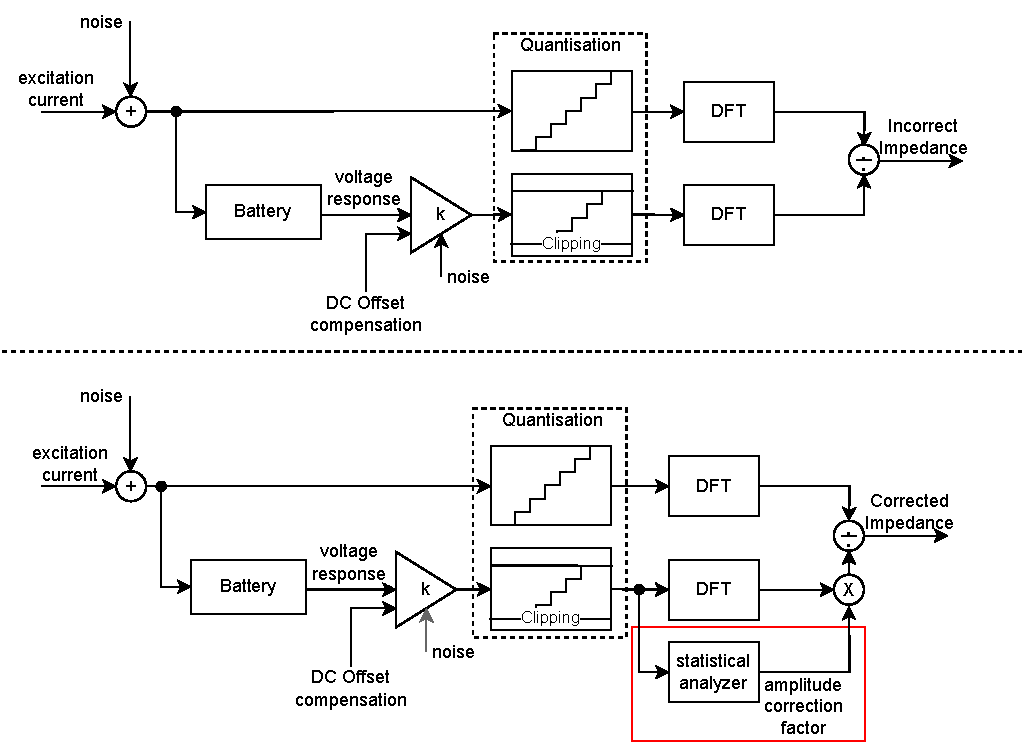
\includegraphics[width=1\textwidth]{../img/system.pdf}
	\caption{Die Berechnung der Impedanz wird infolge von unbekannter Amplitude und Rauscheinflüssen verfälscht, wenn eine Sättigung des ADC eintritt (oben). Zielstellung des vorgestellten Verfahrens ist, die Verfälschung durch einen Amplitude-Korrekturfaktor weitgehend auszugleichen (unten).}
	\label{fig:system}
\end{figure*}

\section{Systemkontext}
Im Batterie-Management-System (BMS) des Fahrzeugs sind komplexe Rechenmodelle für die Zustandsbestimmung der Batterie implementiert. Sie sollen zukünftig auch auf die Impedanzwerte bei verschiedenen Anregefrequenzen zurückgreifen können. Hiervon sollen wertvolle Informationen wie Ladezustand, Temperatur, Alterungszustand und Strombelastbarkeit abgeleitet werden. Die Impedanzwerte sind komplexe Größen, welche sich aus den Wechselgrößen von Strom und Spannung errechnen lassen. Hierzu wird ein Wechselstrom mit einer bestimmten Frequenz als Anregung durch die Reihenschaltung der Zellen geleitet. Über jeder Zelle fällt eine resultierende Spannungsantwort ab. Deren Amplitude vom ohm'schen Anteil des Innenwiderstands der Zellen bestimmt, die Phase von den kapazitiven Effekten beeinflusst. Es sind Rechenmodelle auf der Basis von Ersatzschaltbildern mit mehreren RC-Gliedern üblich~\cite{KeilJossen-2012}.

\smallskip
Bei der Impedanzberechnung werden die Messdaten von Strom und Spannung blockweise ausgewertet, in der Regel erfolgt dies nach Transformation in den Frequenzbereich. Die Abb.~\ref{fig:system} zeigt den Messvorgang im Überblick, dabei bestehen folgende Rahmenbedingungen: Die Messung des Anregestroms im Bereich einiger Ampere wird als messtechnisch weniger problematisch eingeschätzt. Die erforderliche Genauigkeit im Prozentbereich ist mit vertretbarem Aufwand erreichbar. Vereinfachend wird für den Anregestrom von einem nicht übersteuerten Messsignal ausgegangen. Dies gilt nicht für den Messbereich der Spannungsantworten. Die niederohmigen Zellen erfordern hohe Verstärkungsfaktoren, welche zudem an das aktuelle Signal angepasst werden. Dies erfolgt mithilfe einer stufenweise Steuerung des Vorverstärkers durch die nachgeschaltete digitale Signalverarbeitung. Die Voruntersuchungen zeigen, dass im Gegensatz zur Strommessung ist von einem sehr ungünstigen Störabstand auszugehen. Unter diesen Bedingungen ergeben sich in der Regel zahlreiche Abtastpunkte, welche sich im oberen und unteren Sättigungsbereich der Analog-Digital-Umsetzung liegen.

\begin{figure}[t!] 
	\centering
	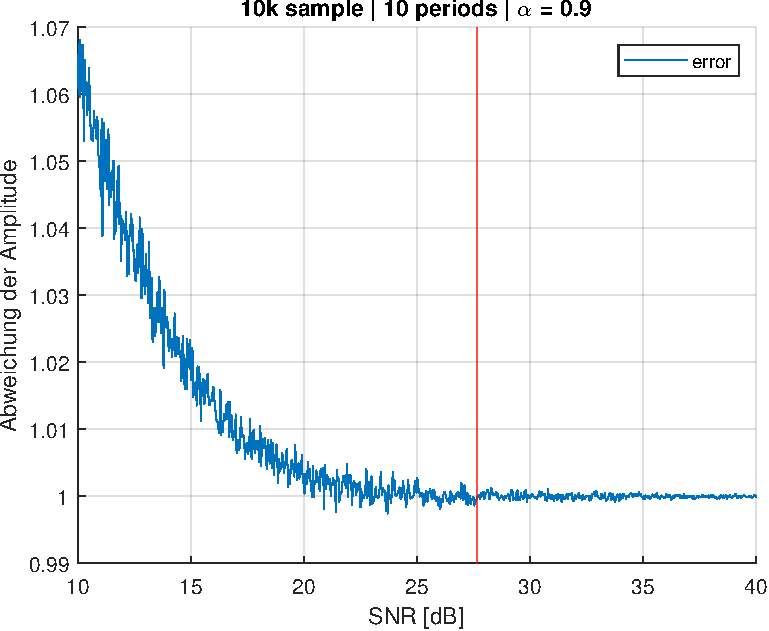
\includegraphics[width=1\columnwidth]{../img/noise-err.pdf}
	\caption{Rauschanteile bewirken eine Abweichung in der berechneten Amplitude.}
	\label{fig:Rauschanteil}
\end{figure}

Die Abb.~\ref{fig:Rauschanteil} zeigt, dass schon durch Sättigung des ADC nur durch Rauschanteile des Signals die berechnete Amplitude verfälscht wird, obwohl die Signalamplitude ohne Rauschen noch nicht übersteuert ist. Ob sich der ADC in Sättigung befindet und inwieweit die Amplitude verfälscht ist, kann durch eine Klirrfaktoranalyse festgestellt werden. Sie ist jedoch vergleichsweise rechenaufwendig. Wenn sich die Ableitung des gemessenen Signals abschnittsweise zu null ergibt, kann eine Aussage über den Grad der Übersteuerung getroffen werden. Bei starken Rauschanteilen ist diese Methode ungeeignet. Auch das einfache Betrachten der Minimal- und Maximalwerten im ADC kann für eine Beurteilung des Sättigungszustands des ADC eingesetzt werden.
Weiterhin ist es für eine optimale Aussteuerung notwendig, dass sich die Abtastwerte des Signals möglichst symmetrisch im Dynamikbereich des ADC verteilen. Dies wird ebenfalls durch das Zusammenwirken von analoger und digitaler Signalverarbeitung sichergestellt. Das vorgestellte Verfahren lässt eine Auswertung der Symmetrie der blockweise erfassten Messwerte zu und steuert damit die erforderliche Referenzspannung, welche von der veränderlichen Zellspannung subtrahiert wird. Diese Kompensierung muss trotz vergleichsweise großer Spannung hinreichend präzise erfolgen, da anschließend hohen Verstärkungsfaktoren verwendet werden.

\section{Lösungsansatz}

Der Lösungsansatz besteht in der stochastischen Auswertung der Verteilung der Datenpunkte des Signals. Mit den gemessenen Charakteristiken wird ein Rückschluss auf den Grad des Fehlers der Messung ermöglicht. Entsprechende Amplitude-Korrekturfaktoren (AKF) können zur Korrektur angewandt werden. Das Histogramm wird in $h_b = 2^n$ mit $n = 12$ Klassen aufgeteilt, dies entspricht den Quantisierungsstufen des ADC. Die Ränder $h_0$ und $h_b$ beinhalten die Datenpunkte in den Grenzbereichen des Dynamikumfanges des ADC. Über den Anteil der Datenpunkte, welche sich in den Randbereichen befinden, lässt sich eine Aussage über den Sättigungsgrad des ADC treffen. In Kombination mit den stochastischen Momenten Varianz und Kurtosis kann der Fehler, welcher durch Sättigung des ADC entsteht, einem AKF zugeordnet und anschließend kompensiert werden.  

\section{Statistische Analyse}

Das Histogramm findet unter anderem Anwendung zum Testen und zur Charakterisierung von Analog-Digital-Wandlern~\cite{Gamad-2009}. Sinusförmige Signale weisen eine charakteristische Verteilungsfunktion auf, welche qualitativ einem Spezialfall der Beta-Verteilung für $\alpha = \beta$ entspricht. In der Abb.~\ref{fig:Histogramm-Gain} (oben) ist die charakteristische Ausprägung des Histogramms eines periodengenauen, sinusförmigen Signals für steigende Verstärkungen zu sehen. Zu erkennen ist, dass die Datenpunkte sich bei zunehmender Verstärkung des Signals in die Randbereiche verlagern. Der Anteil der sich in Sättigung befindlichen Abtastwerte wird im folgenden Sättigungsgrad $c$ genannt. Auch durch die statistischen Momente der Verteilung beeinflusst. Dazu gehören Varianz und Kurtosis (Wölbung).
\begin{figure*}[h!] 
	\hspace*{-2mm}
	\centering 
	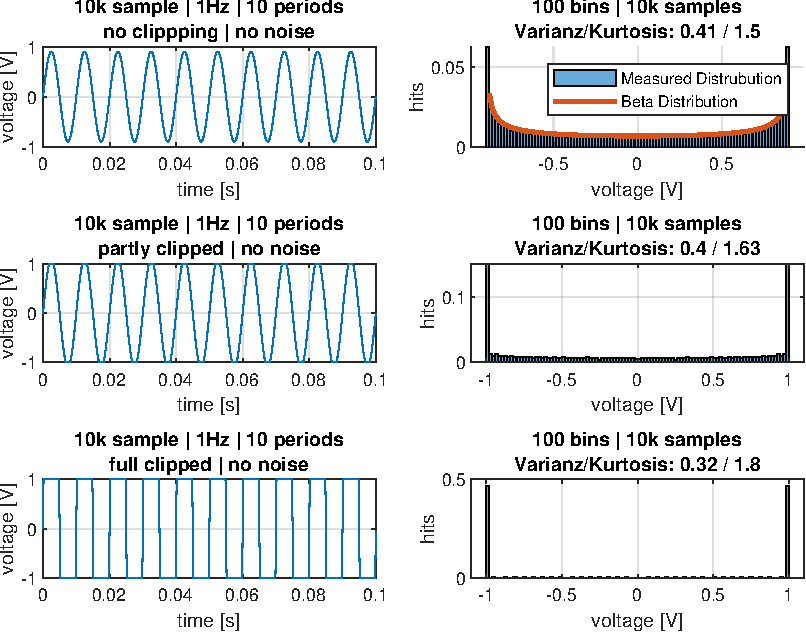
\includegraphics[width=1.05\columnwidth]{../img/beta-distribution.pdf}~~~~~
	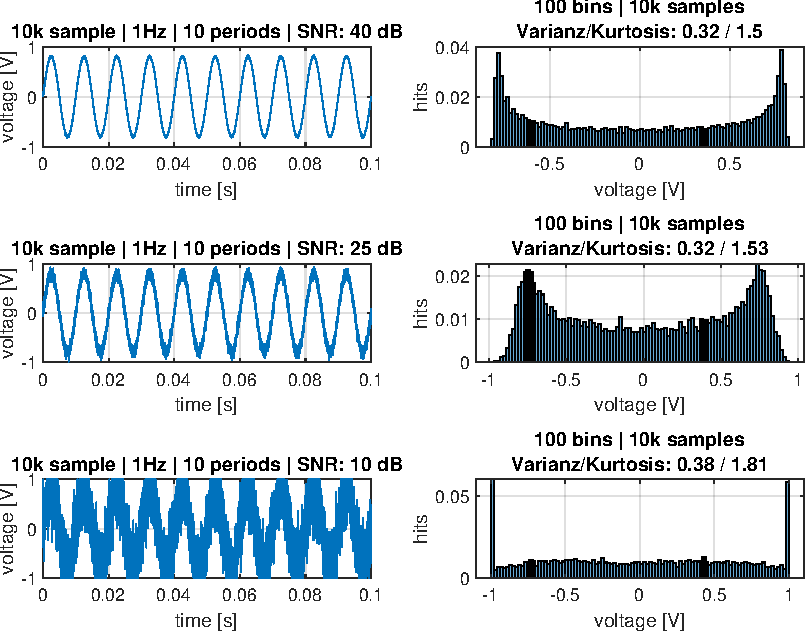
\includegraphics[width=1.05\columnwidth]{../img/noise-histogramm.pdf}
	\caption{Die linken Histogramme werden durch rauschfreie Signale mit verschiedener Amplitude erzeugt. Dabei werden unterschiedliche Sättigungsgrade dargestellt. Die rechten Histogramme zeigen verschiedene Rauschverhältnisse bei konstanter Amplitude.}
	\label{fig:Histogramm-Gain}
\end{figure*} 
Die Abb.~\ref{fig:Histogramm-Gain} (unten) zeigt den Verlauf des Histogramms bei zunehmendem Rauschen (Verschlechterung des SNR) und konstanter Verstärkung. Im Vergleich zu einem rauschfreien sinusförmigen Signalverlauf bildet sich das Histogramm weniger markant aus. Die Datenpunkte verteilen sich gleichförmiger über alle Klassen des Histogramms, bis die Sättigung durch starkes Rauschen wieder zu einer Konzentration der Datenpunkte in den Randbereichen führt. Auffällig ist außerdem, dass die Varianz mit steigendem Sättigungsgrad des ADC wenig Veränderung aufweist, wohingegen die Kurtosis sensitiver reagiert. Das Histogramm ist durch einfaches Zählen der Abtastpunkte im Wertebereich einer Klasse zu implementieren. Es kann verwendet werden, um Rückschlüsse auf die Signalqualität des vorliegenden Signals zu ziehen und um Korrekturen von Verfälschungen zu ermöglichen. 


\section{Ermittlung der Korrekturfaktoren}
Der Zusammenhang der Korrekturfaktoren wird über den Störabstand und der Verstärkung des Signals mit den drei angeführten Größen: 
\begin{itemize}
	\item Sättigungsgrad als Anteil der Datenpunkte in der Sättigung des ADC
	\item Varianz der Verteilung der Abtastwerte\footnote[1]{Nicht berücksichtigt werden Abtastwerte in der Sättigung des ADC.\label{foot:bereinigt}}
	\item Kurtosis der Verteilung der Abtastwerte\footref{foot:bereinigt}
\end{itemize}

Der Sättigungsgrad ergibt sich aus der Anzahl der Datenpunkte in den äußersten Klassen $h_0$ und $h_b$ des Histogramms nach Gl.~\eqref{eq:dist_sat}. Der Dynamikbereich des ADC wird bei 12-Bit in $b=4096$ Stufen aufgelöst. Jeder Datenpunkt kann in einem Histogramm einer Klasse $b_i$ zugeordnet werden.

\begin{equation}
	\label{eq:dist_sat}
	c = h_0 + h_b = \frac{n_0 + n_b}{n} \cdot 100
\end{equation}

Die Ermittlung der AKF muss zuvor mittels Simulation experimentell erfolgen. 
Dafür wird in der Simulation ein sinusförmiges Referenzsignal $u_{Ref}(t)$ mit bekannter Amplitude verwendet, dass kein Rauschen aufweist. Spektralanteile außerhalb der Grundfrequenz $f_0$ des Referenzsignals werden nicht betrachtet. 
Dieses Signal $u_{Ref}(t)$ wird außerdem mit additivem Rauschen beaufschlagt, entsprechend dem Batteriemodell beeinflusst und multiplikativ verstärkt. Anschließend wird es in den Minimal- und Maximalwerten begrenzt und quantisiert. Hierfür werden für die relevanten Kombinationen aus SNR $n$ und Verstärkung $g$ durchlaufen. Es ergibt sich das Signal $u_{n,g}(t)$. Dafür wird jeweils der Sättigungsgrad des ADC, die Varianz $\sigma^2(u_{n,g}(t))$ und die Kurtosis $w(u_{n,g}(t))$ bestimmt.
Für den AKF ergibt sich im Frequenzbereich Gl.~\eqref{eq:corr}.

\begin{equation}
	\label{eq:corr}
	AKF_{n,g} = \frac{|\hat{U}_{Ref}(f_0)|}{|\hat{U}_{n,g}(f_0)|}
\end{equation}

Zur weiteren Optimierung kann der Korrekturfaktor auch komplex bestimmt werden, der aktuelle Ansatz verwendet den Betrag und skaliert den Imaginär- und Realteil der komplexen Amplitude.

\begin{figure*}[h!]
	\centering
	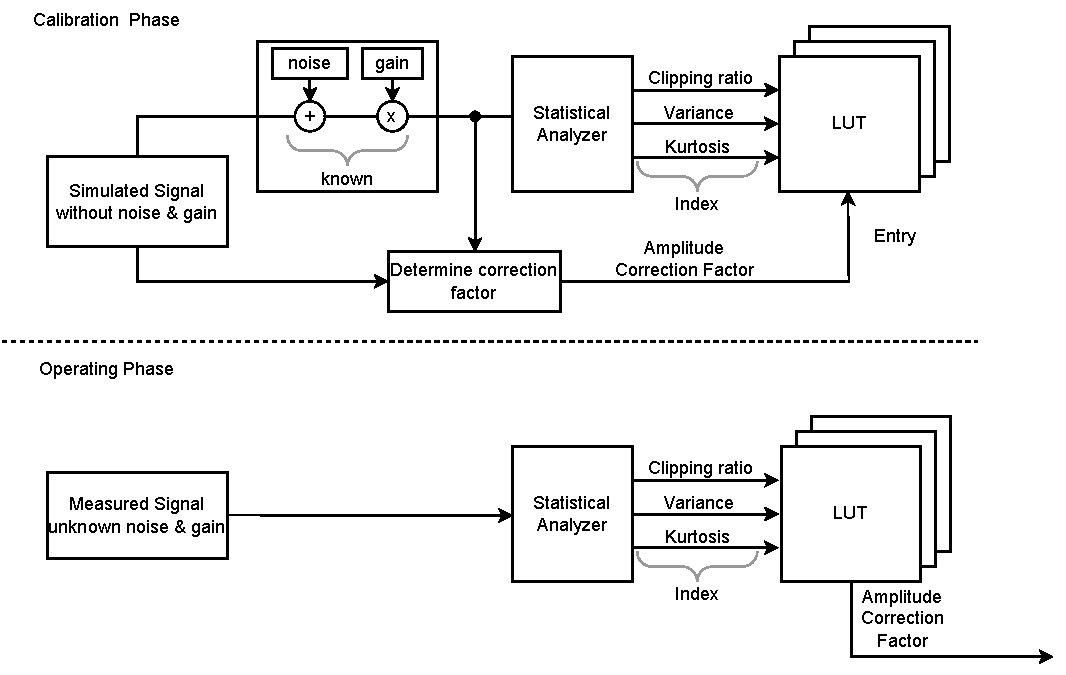
\includegraphics[width=.85\textwidth]{../img/factor.pdf}
	\caption{Während der Kalibrationsphase wird die LUT erstellt. Während der Messung liefert die LUT den Amplituden-Korrekturfaktor.}
	\label{fig:factor_eval} 
%\end{figure*}
%
%\begin{figure*}[h!]
	\centering
	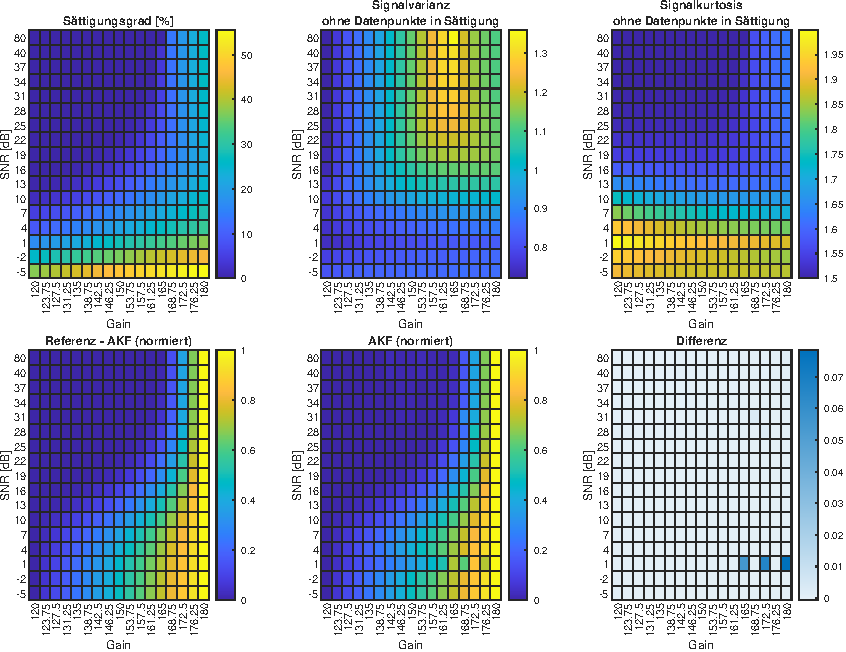
\includegraphics[width=.85\textwidth]{../img/lut.pdf}
	\caption{Die stochastischen Merkmale der Verteilung (oben) werden verwendet, um auf die Signalqualität zu schließen. Die AKF (unten) werden für jede Kombination von Verstärkungsfaktoren und Rauschabstand gebildet des Signals gebildet. In den Darstellungen (oben) ist zu erkennen, dass der Sättigungsgrad, die Varianz und die Kurtosis unterschiedliche Bereiche mit deutlichen Gradienten aufweisen. Diese Bereiche ergänzen sich in der Überdeckung. Damit wird eine Zuordnung mit hinreichender Sicherheit möglich, wenn diese drei Parameter herangezogen werden.}
	\label{fig:lut} 
\end{figure*}

\begin{figure*}[t!]
	\centering
	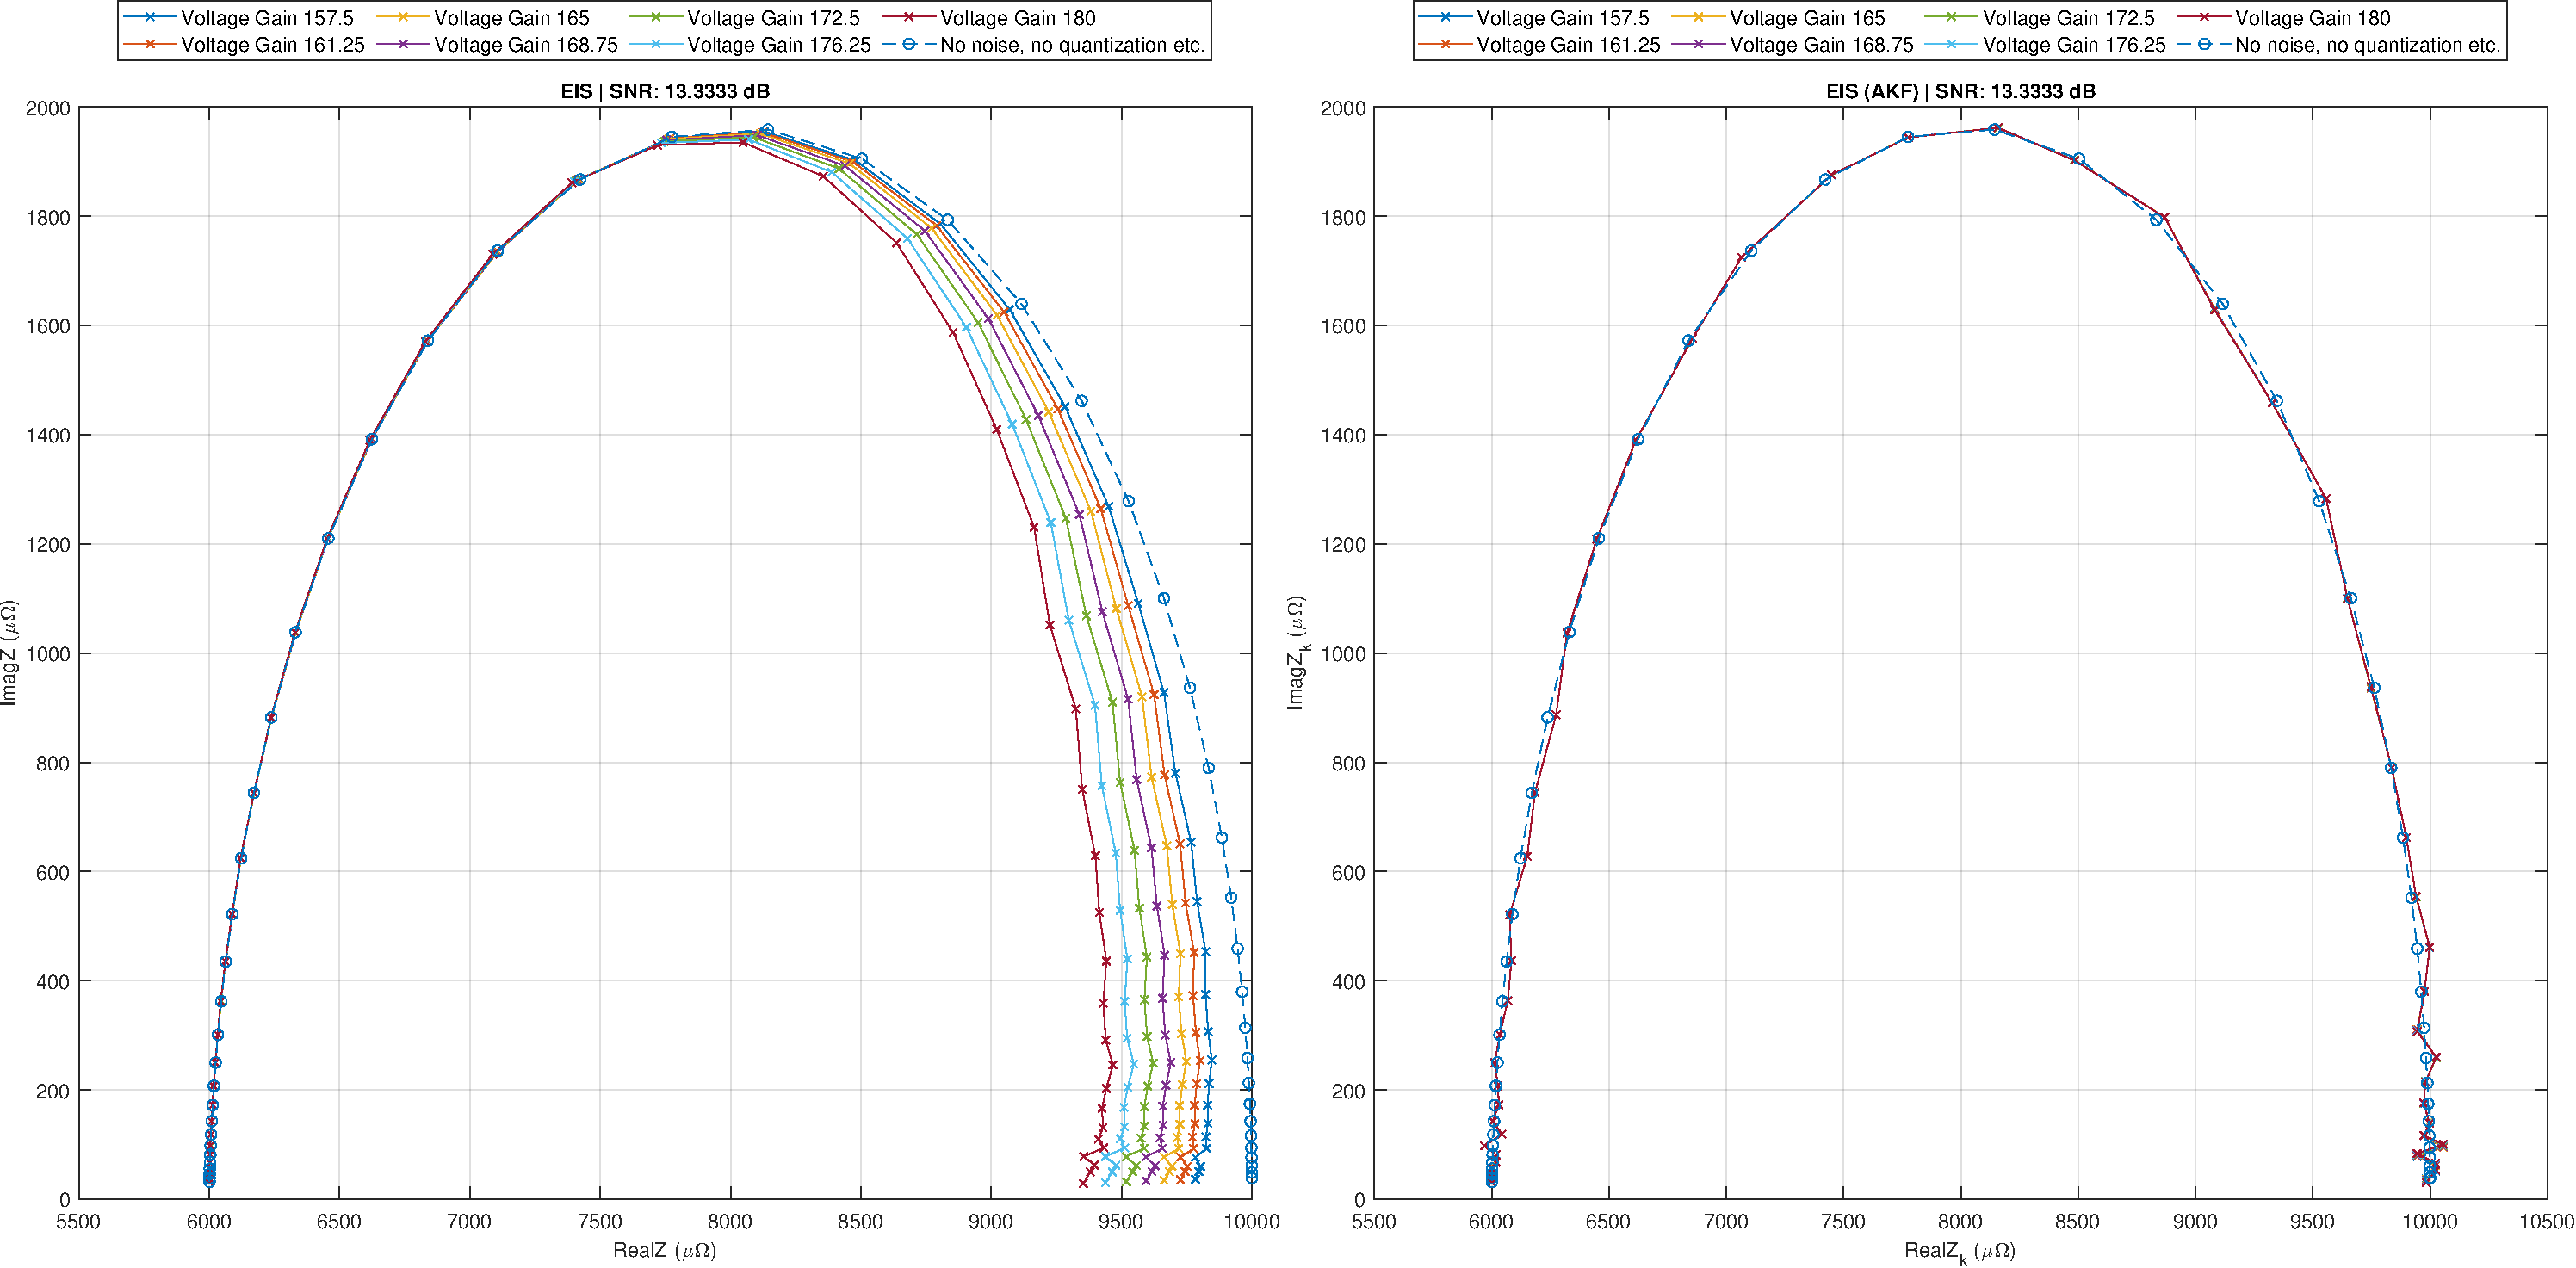
\includegraphics[width=.9\textwidth]{../img/ergebnisse.pdf}
	\caption{Das EIS-Spektrum weist nach der Korrektur eine deutliche Verbesserung im direkten Vergleich auf. Die Korrektur ist besonders bei hohen Verstärkungen wirksam, was auf den Amplitudengang des Batteriemodells zurückzuführen ist.}
	\label{fig:Ergebnisse} 
\end{figure*}

\section{Kalibrations- und Nutzungsphase}

Zunächst wird Kalibrationsphase durchgeführt, in welcher eine Zuordnung des AKF anhand der statistischen Eigenschaften des Ausgangssignals erfolgt. Diese Zuordnung wird als tabellarische Abbildung in einer Look-Up Tabelle (LUT) gespeichert, siehe Abb.~\ref{fig:factor_eval}. 
Die Einträge der LUT werden durch Simulationsläufe für die Kombinationen der Parameter Verstärkung und Rauschanteil erzeugt. Dabei durchlaufen die Parameter stufenweise Bereiche, die für die Anwendung zuvor abgeschätzt wurden. Sofern dabei Einträge der LUT nicht besetzt werden, erfolgt eine Interpolation.
Die Mehrfachbesetzung von Einträgen in der LUT kam in der Simulation selten vor, in diesem Fall wurde der vorherige Eintrag überschrieben. Der resultierende Fehler hat einen vernachlässigbaren Einfluss. Dies entspricht auch der geringen Abweichung in der Differenzdarstellung in Abb.~\ref{fig:lut} (unten rechts). 

In der späteren Nutzungsphase kann das Messsignal nach den statistischen Eigenschaften blockweise analysiert werden. Die drei Ergebnisse der Analyse können unmittelbar als Index der LUT verwendet werden und der AKF unmittelbar aus der LUT ausgelesen werden. Die Abb.~\ref{fig:lut} zeigt die Charakteristik des Sättigungsgrades und der stochastischen Momente für die Signale $u_{n,g}(t)$. Als Alternative zur LUT kann eine Funktion von drei Variablen verwendet werden. Die Koeffizienten einer Linearkombination von $c$, $\sigma^2$ und $w$ wurde durch numerische Optimierung bestimmt und zeigten vergleichbare Ergebnisse.

\smallskip
\section{Simulationsexperiment}
Zunächst werden die AKF in der Simulation\footnote[2]{Der Quellcode zur Simulation: https://github.com/TobiasFrahm/histogramm-verfahren} berechnet. Hierfür wurde der in Abb.~\ref{fig:factor_eval} dargestellte Signalfluss implementiert. Das Stromsignal wird vor der Berechnung der Spannungsantwort mit additivem weißem Rauschen beaufschlagt. Das verwendete Batteriemodell ist ein einfaches RRC-Modell ($R0 = \SI{6}{m\Omega}, R1=\SI{4}{m\Omega}, C1=\SI{500}{mF}$), damit wurde die Spannungsantwort transient berechnet. Der Rauscheinfluss am Verstärker wurden in dem Simulationsexperiment vereinfachend nicht berücksichtigt. Die Anregung erfolgt mit einer Amplitude von $\SI{1}{A}$, der erwartete Wechselanteil der Spannungsantwort liegt bei ca. $\SI{10}{mV}$. Der durch die Batteriespannung aufgeschlagene Gleichanteil der Spannungsantwort wird subtrahiert. Die Quantisierung erfolgt mit einem Dynamikbereich von $12$-Bit, die Sättigung des ADC wird durch die Limitierung der Werte simuliert. Die Grenzwerte liegen für das Minimum bei $\SI{0}{V}$ und im Maximum bei $\SI{3.3}{V}$. Die Verarbeitung der Signale erfolgt blockweise mit $10000$ Abtastwerten. Für die Bildung der AKF wird die Simulation für den Wertebereich der Verstärkung $g = 120 ... 180$ und dem Störabstand $n = -5 ... \SI{80}{dB}$ durchgeführt. In der Nutzungsphase wird die EIS berechnet, dabei wird auf die vorberechnete LUT zugegriffen. Der dort entnommene AKF wird multiplikativ mit der Amplitude im Frequenzbereich verrechnet, Gl.~\eqref{eq:corr_mat}. Zur Validierung wurden die vorgenannten Bereiche der Verstärkung und des Störabstands durchlaufen und jeweils die EIS bestimmt.

\begin{equation}
	\label{eq:corr_mat}
	Z_k(f) = \frac{\hat{U}_{n,g}(f_0) \cdot AKF}{\hat{I}(f_0)}
\end{equation}	


\section{Ergebnisse und Diskussion}
Die Ergebnisse in Abb.~\ref{fig:Ergebnisse} zeigen eine deutliche Verbesserung in der Berechnung der EIS. Es werden in der Abbildung die Nyquist-Plots des einfachen RRC-Modells dargestellt, die einen Halbkreis in der komplexen Darstellung bilden. 
Die Berechnung der EIS weist ohne Korrektur (links) im niederfrequenten Bereich, das heißt mit hohem Realteil in der Impedanz, einen ausgeprägten Fehler auf. Hier wirkt sich der Amplitudengang des Modells aus. Der Fehler zeigt sich in einer sättigungsabhängigen Stauchung des Halbkreises im Nyquist-Plot. Für die Bereiche des Simulationsexperiments sind bis zu $10\%$ verfälschte Impedanzwerte aufgetreten. Dieser Fehler kann mit dem vorgeschlagenen Korrekturverfahren erheblich vermindert werden, er reduziert sich auf etwa $1\%$. 

\smallskip
Die Abb.~\ref{fig:Ergebnisse} (unten rechts) zeigt den prozentualen Sättigungsgrad in Abhängigkeit der Verstärkung der Spannung. Das Korrekturverfahren ist bei minimalem Sättigungsgrads nicht erforderlich. Es sollte dann nicht angewandt werden, weil es ggf. zu einem geringen zusätzlichem Fehler führen kann, siehe Abb.~\ref{fig:Ergebnisse} (unten links). 

Eine statistische Analyse der Abtastwerte ist bereits in zur Steuerung der Vorverstärkung verwendet worden~\cite{Frahm-2023}. Die vorgestellte Methode zur Korrektur der Sättigung geht darüber hinaus, sie sind zunächst in Simulationsexperimenten untersucht worden. Das Verfahren wird gegenwärtig auf Mikrocontrollern im Rahmen der Entwicklung von Batteriezellsensoren umgesetzt. Das Gesamtziel des Forschungsprojekts ist gemeinsam mit Projektpartnern die elektrochemische Impedanzspektroskopie als Messmethode für große Fahrzeugbatterien in Elektrofahrzeugen verfügbar zu machen.

\section*{Förderung}
Die Untersuchung entstand im Rahmen des Verbundprojekts ProMoBiS - "Progressive Multizell-Verbund-Konzepte für Batteriesysteme mit integrierter Sensorik". Das Forschungsprojekt wird vom Bundesministerium für Wirtschaft und Klimaschutz (BMWK) im Rahmen des 7. Energieforschungsprogramms (Förderkennzeichen 03ETE046G) im Bereich "\,Energiewende im Verkehr"\,gefördert und vom Projektträger Jülich betreut.
   
\begin{thebibliography}{[99]}

	\bibitem{Schmidt-2013}
	Schmidt, Jan Philipp, "Verfahren zur Charakterisierung und Modellierung von Lithium-Ionen Zellen" , Dissertation, Karlsruhe, KIT Scientific Publishing, 2013.
	
	\bibitem{KeilJossen-2012}
	P. Keil und A. Jossen, "\href{https://mediatum.ub.tum.de/doc/1162416/1162416.pdf}{Aufbau und Parametrierung von Batteriemodellen}", 19. DESIGN\&ELEKTRONIK-Entwicklerforum Batterien \& Ladekonzepte, München, 2012.
	
	\bibitem{Roscher-2016}
	V. Roscher. K.-R. Riemschneider. N. Sassano, "Batterie-Zellensensoren mit drahtloser Kommunikation und verteilter Signalverarbeitung" in Automobil-Sensorik, T. Tille, Hrsg., Springer, 2016.
	
	\bibitem{Hammerschmidt-2016}
	T. Hammerschmidt, J.P. Schmidt, "Impedanzsensorik für Batteriezellen in Elektro-Fahrzeugen" in Automobil-Sensorik, T. Tille, Hrsg., Springer, 2016.
	
		
	\bibitem{Abel-1991}
	J. S. Abel and J. O. Smith, III, "Restoring a clipped signal" in
	Proc. IEEE ICASSP, pp. 1745–1748, 1991. 
	
	\bibitem{Ting-2013}
	S. -K. Ting and A. H. Sayed, "Mitigation of clipping in sensors" IEEE International Conference on Acoustics, Speech and Signal Processing, pp. 5934-5938, doi: 10.1109/ICASSP.2013.6638803, 2013.
	
	\bibitem{Zhou-2019}
	N. Zhou, J. Wang, B. Sun, R. Liu and N. Hu, "The Automatic Repairing Method Addressing Clipping Distortions and Frictional Noises in Electronic Stethoscope" IEEE 7th International Conference on Bioinformatics and Computational Biology (ICBCB), pp. 195-199, doi: 10.1109/ICBCB.2019.8854669, 2019.
	
	\bibitem{Chan-2012}
	A. D. C. Chan. J. R. Green. D.Maclsaac. G. D. Fraser, "Detection of ADC clipping, quantization noise, and amplifier saturation in surface electromyography" IEEE International Symposium on Medical Measurements and Applications Proceedings, 2012.
	
	\bibitem{Jung-1993}
	P. Jung, "Periodically driven stochastic systems", Physics Reports,  pp. 175-295, 1993.

	\bibitem{Gamad-2009}
	R.S. Gamad, D.K. Mishra,
	"Gain error, offset error and ENOB estimation of an A/D converter using histogram technique",
	Measurement, Volume 42, Issue 4, pp. 570-576, https://doi.org/10.1016/j.measurement.2008.10.003, 2009.

	\bibitem{Frahm-2023}
	T. Frahm "\,Sensorsystem für die Impedanzspektroskopie in Fahrzeugbatterien: Analogvorstufe, Signalverarbeitung und Software", Masterarbeit, HAW Hamburg, 2023.


	
\end{thebibliography}
	

 
\end{document} 